\documentclass{article}

% if you need to pass options to natbib, use, e.g.:
% \PassOptionsToPackage{numbers, compress}{natbib}
% before loading nips_2017
%
% to avoid loading the natbib package, add option nonatbib:
% \usepackage[nonatbib]{nips_2017}
\PassOptionsToPackage{numbers, compress}{natbib}
%\usepackage{nips_2017}

% to compile a camera-ready version, add the [final] option, e.g.:
\usepackage[final]{nips_2017}
\usepackage[utf8]{inputenc} % allow utf-8 input
\usepackage[T1]{fontenc}    % use 8-bit T1 fonts
\usepackage[hyphens]{url}            % simple URL typesetting
\usepackage{hyperref}       % hyperlinks; must be after url for line breaks to work
\usepackage{booktabs}       % professional-quality tables
\usepackage{amsfonts}       % blackboard math symbols
\usepackage{nicefrac}       % compact symbols for 1/2, etc.
\usepackage{microtype}      % microtypography
\usepackage{color}
\usepackage{subcaption}

\usepackage{graphicx}
\graphicspath{{./images/}}

\bibliographystyle{abbrvnat}
%\PassOptionsToPackage{square, sort, numbers}{natbib}


\title{Real-Time Object Detection Using Low-Cost Hardware}

\author{
    \textbf{Xiaolan Cai}$^\text{1}$, 
    \textbf{Warren Ferrell}$^\text{1}$,
    \textbf{Chu-Sheng Ku}$^\text{1}$,
    \textbf{Soham Shah}$^\text{1}$,
    \textbf{Ryan Skinner}$^\text{2}$
    \\
    $^\text{1}$Department of Computer Science\\
    $^\text{2}$Department of Aerospace Engineering Sciences\\
    University of Colorado at Boulder\\
    Boulder, CO 80309
}

\begin{document}
% \nipsfinalcopy is no longer used

\maketitle
\begin{abstract}
We investigate the feasibility of real-time object detection using the YOLO algorithm on low-cost platforms. Towards this end, we vary the design of YOLO's neural network and implement various hardware optimizations while running it on a Raspberry Pi. We find that it remains difficult to classify objects faster than approximately 1 fps on a Pi CPU, but that lowering the number of object classes and replacing the network head with a MobileNet architecture results in a favorable accuracy-to-cost trade-off. Ultimately, we conclude that our design modifications coupled with a low-cost mobile GPU such as Intel's Movidius Neural Compute Stick or Nvidia's Jetson hardware would make real-time object detection feasible.
\end{abstract}

\section*{Contributions}
\begin{tabbing}
XXXXXXXXX \= \kill% this line sets tab stop

Xiaolan Cai \> Implement mAP evaluation scripts on validation data, theory-thinking\\

Warren Ferrell \> Setup personal laptop server the for team to make use of GPU, network training,\\ \> created utilities for accuracy scripts, and produced final mAP graphs \\

Chu-Sheng Ku \> Setup YOLO with Darknet, Darknet NNPACK and MobileNet on \\ \> Raspberry Pi, real-time demonstration on MacBook Pro\\

Soham Shah \> Set up Darknet + YOLO on the Raspberry Pi, optimized Darknet to run on the\\ \> Raspberry Pi\\

Ryan Skinner \> Caltech/KITTI data pre-processing and sampling, Boulder video acquisition and\\ \> evaluation, theory-thinking, network training, and \LaTeX-wrangling
\end{tabbing}

\section{Introduction}
As autonomous vehicles become increasingly integrated into our everyday life, it is critical that these vehicles are able to operate effectively and safely in any environment. One of the key challenges in building fully autonomous self-driving cars is being able to identify and track objects near the vehicle. On the other hand, an important aspect of self-driving car proliferation will be taking robotics research and making it usable in real-world production environments, and especially on low-cost platforms. In the case of small autonomous vehicles, the question of sufficient computational resources for object detection becomes an even greater concern. 

Many hobbyists have adopted the Raspberry Pi as their micro-controller of choice, as it has a good amount of computational power and can interface with numerous sensors at a low price. In this project, we build and train our own you-only-look-once (YOLO) neural network to recognize images relevant to an autonomous vehicle. Two approaches are taken to reduce the cost of network evaluation: altering the network design, and optimizing its hardware implementation on a Raspberry Pi.

\section{Materials and Methods}
\label{materials_and_methods}

\subsection{YOLO Algorithm}

\begin{figure}[t]
  \centering
  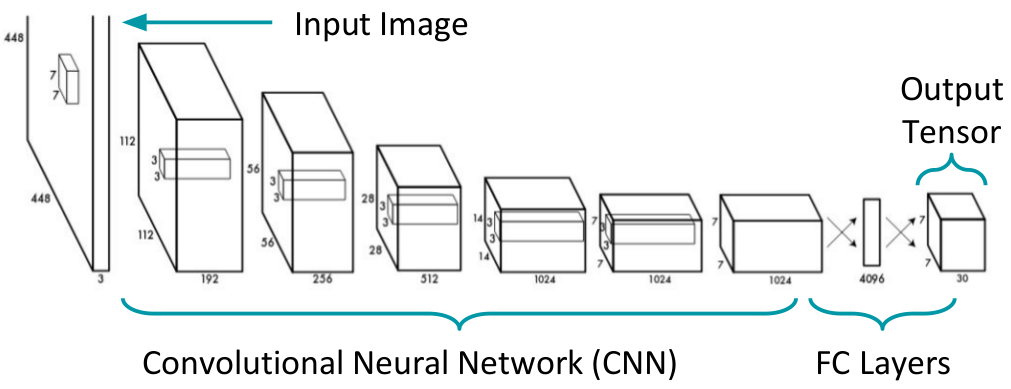
\includegraphics[width=0.5\textwidth]{yolo_diagram}
  \caption{Schematic diagram of the YOLO network.}
  \label{fig:yolo}
\end{figure}

We begin by describing the YOLO algorithm, which consists of a feed-forward artificial neural network (ANN) and a post-processing algorithm called non-max suppression (NMS). The ANN architecture is shown in Figure~\ref{fig:yolo}. The input image is fed into a convolutional neural network (CNN) which extracts features from the image. The authors of YOLO provide two versions of the CNN: ``Full'' and ``Tiny''. These are simple stacks of conv-pool layers, with Full-YOLO having on the order of 30 and Tiny-YOLO having around 9.

The features extracted by the CNN front-end are passed through a set of fully-connected layers to an output tensor. The output tensor is the most complex part of the algorithm, and its interpretation is as follows. First, the output tensor has dimension
\begin{equation}
    S \times S \times (B \times (5 + C))
    \label{eq:tensordim}
\end{equation}
where the input image is divided into an $S \times S$ grid, $B$ is the number of anchor boxes used by the algorithm, and $C$ is the number of object classes that can be detected. Note that this four-tensor can be interpreted as a three-tensor or volume by flattening the indices of the outermost parentheses of (\ref{eq:tensordim}) into one dimension. This eases implementation in libraries such as TensorFlow.

Each anchor box has a unique aspect ratio and allows for detection of overlapping objects in the same grid cell. If there were only a single anchor box ($B=1$), YOLO could detect at most one object per cell in the $S \times S$ grid. Furthermore, anchor boxes allow for higher accuracy when detecting objects of disparate aspect ratios. For example, a person is tall and skinny, whereas a car viewed obliquely may be short and wide. The first five values are associated with each anchor box are the probability $P_{obj}$ of an object being in that anchor box, and the bounding box coordinates ($b_x$, $b_y$) and dimensions ($b_w, b_h$). The next $C$ values are the probabilities of the object belonging to a particular class ($P_{c_1}$, $P_{c_2}$, ... $P_{c_C}$).

During training, the loss function always uses $P_{obj}$. However, the loss function ignores all other bounding box parameters and class probabilities when false positive detections occur. Thus the existence of $P_{obj}$ gives the algorithm a certain degree of flexibility, allowing box and class predictions to be trained only on instances where there are truly objects.

When detecting objects, the practitioner sets a threshold for $P_{obj}$ below which bounding box predictions are ignored. We experimented and found values between 0.3 and 0.4 to produce good results. As will be shown later, precision-recall plots are generated by sweeping the threshold for $P_{obj}$; an optimal threshold can be chosen based on these plots. Just placing a threshold on $P_{obj}$ is not enough, however, as many bounding boxes may be generated for a given object, each with slightly different coordinates and sizes.

This motivates the last part of the YOLO algorithm: non-max suppression (NMS). In this final step, for each class $c_j$, the bounding box with the highest value of the class confidence $P_{c_j}$ is selected. Then all bounding boxes that are associated with $c_j$ and overlap enough (as measured by the boxes' intersection over union, IoU) are deleted. This process repeats until no boxes of the same class have an IoU greater than the chosen threshold. An example of the NMS procedure is shown in Figure~\ref{fig:nms}. The boxes remaining after NMS are returned as the output of the YOLO algorithm.

\begin{figure}[t]
  \centering
  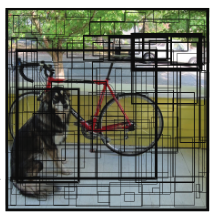
\includegraphics[height=3cm]{yolo_allboxes}
  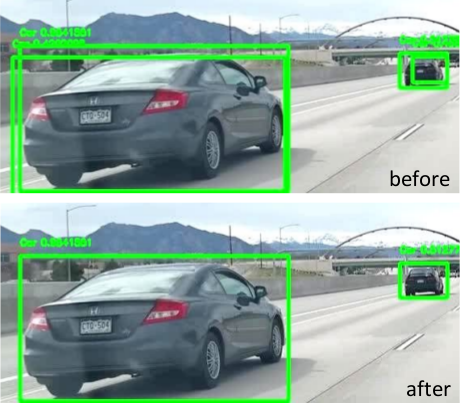
\includegraphics[height=3cm]{nms_diagram}
  \caption{Clockwise from left: Example of all bounding boxes returned by YOLO, prior to NMS, from \cite{YOLO}. Bounding boxes above a given threshold for our dataset, prior to NMS. Output after NMS.}
  \label{fig:nms}
\end{figure}


\subsection{Cost-Reduction by Network Design}

We identified three approaches to reduce the evaluation cost by modifying the design of the YOLO network. The one we did not implement due to complexity and time constraints was replacing the fully-connected layers in the YOLO network with the ConvDet layer described by \cite{wu_convdet}.

The two we did implement are as follows. First, we substantially reduce the size of the fully-connected weights and the output tensor by reducing the number of classes from $C=20$ for the ``default'' YOLO to only $C=1$. Second, we replaced the CNN front-end of the YOLO network with Google's MobileNet architecture provided by Keras.

\begin{figure}[t]
  \centering
  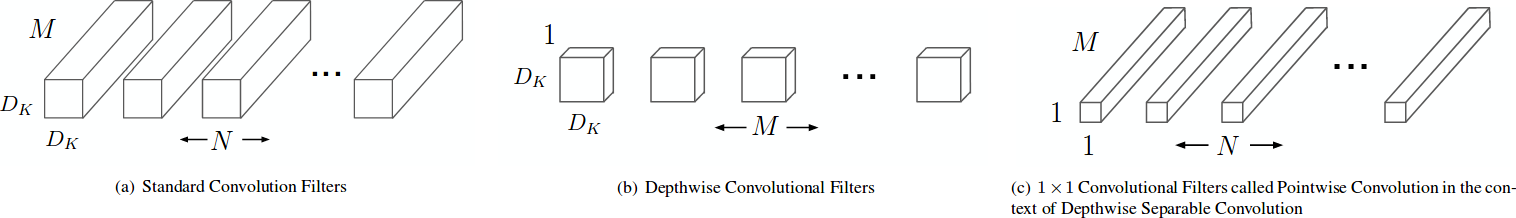
\includegraphics[width=\textwidth]{mobilenet_depthwise_sep}
  \caption{In MobileNet, the standard convolution filters in (a) are replaced by two layers: (b) in-channel depth-wise convolutions (c) cross-channel point-wise convolutions. Image and caption reproduced from \cite{MobileNet}.}
  \label{fig:depthwise_sep}
\end{figure}

MobileNet is an efficient neural network designed for mobile vision applications with hyper-parameters designed to allow for easy tuning of the network for speed or accuracy without the need for costly retraining of the whole network \cite{MobileNet}. MobileNet reduces the number of required multiply-adds required for of a network of its size by a factor of 8 through the use of depthwise separable convolutions, which consist of depthwise convolutional filters and pointwise convolutional filters. As shown in Figure~\ref{fig:depthwise_sep}, this design reduces the size of the convolutional layers of the network from $N$ convolutions of size $M \times D_K \times D_K$ to $M$ depthwise convolutions of size $1 \times D_K \times D_K$ and $N$ pointwise convolutions of size $M \times 1 \times 1$ where $M$ is the number of input channels, $N$ is the number of output channels, and $D_K$ is the dimension of the applied filter. This optimization does reduce the network's accuracy on the ImageNet dataset by 1.1\% but has the benefit of reducing the number of Mult-Adds per evaluation from 4866 million to 569 million.

\begin{figure}[b]
  \centering
  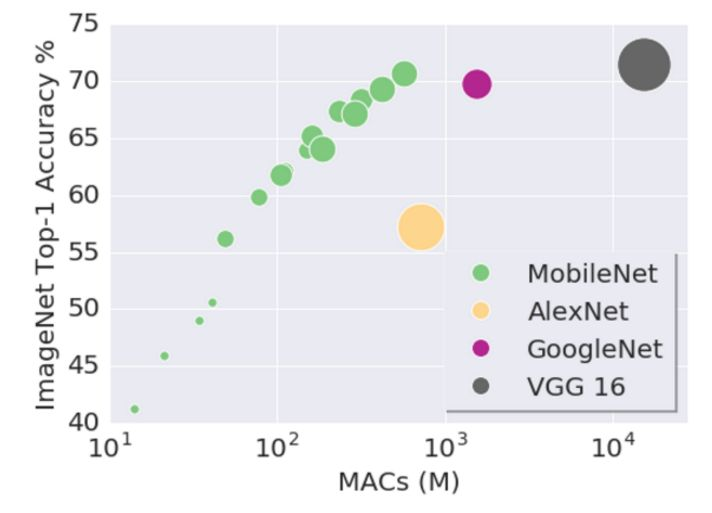
\includegraphics[width=0.4\textwidth]{mobilenet_fig}
  \caption{Compared to standard conv-pool architectures, Google's MobileNet reduces the number of multiply-accumulate operations during network evaluation while maintaining reasonable accuracy. Image from \cite{mobilenetfig}.}
  \label{fig:mobilenet}
\end{figure}

To allow for further optimization of network's feed-forward cost, MobileNet exposes two parameters: the width and resolution multipliers $\alpha$ and $\rho$. These parameters trade accuracy for speed, and result in the multiple MobileNet points shown in Figure~\ref{fig:mobilenet}. The first of these parameters, $\alpha$, scales both the computational cost and number of training parameters roughly quadratically while $\rho$ just reduces the computational cost. 

We performed some promising experiments with these parameters but were unable to get them working in our final architecture due to time constraints. The default MobileNet and what was used in our experiments is the highest accuracy point in Figure~\ref{fig:mobilenet}.

\subsection{Cost-Reduction by Hardware Optimization}

To establish a base case, we took a sample image and the base YOLO algorithm on the Raspberry Pi with Darknet and the pre-trained weights. This gave us a classification time of 150 sec. From there, we started experimenting with ways to speed this process up. The first thing was to use Tiny-YOLO. This is basically using fewer layers in the classification process in order to gain some speed boost. Using this, we still got decently accurate classifications (see above) but at a much faster speed of 38 seconds.

One of the optimizations we explored was ARM\_NEON. NEON is an advanced SIMD (single instruction multiple data) architecture extension that helps with image and video processing. This basically allows for multiple processing elements in the pipeline to perform operations on multiple data point with a single instruction \cite{NEON}.

Another optimization that we explored was NNPACK. Quoting its documentation, ``NNPACK is an acceleration package for neural network computations. NNPACK aims to provide high-performance implementations of convnet layers for multi-core CPUs'' \cite{NNPACK}. This allowed us the parallelize our convolution operations across the cores in the CPU which sped up computation.

Although we could improve our detection speed 6$\times$---from 8.2 seconds to 1.3 seconds for a still image by using NNPACK---it sacrifices accuracy as shown in Figure~\ref{fig:trade-off}. With YOLO, we got detection distribution dog: 81\%, truck: 74\%, bicycle: 83\% in 8.2 seconds; with Tiny-YOLO, we got dog: 78\%, car: 55\%, car: 50\% in 1.3 seconds.

\begin{figure}[t]
  \centering
  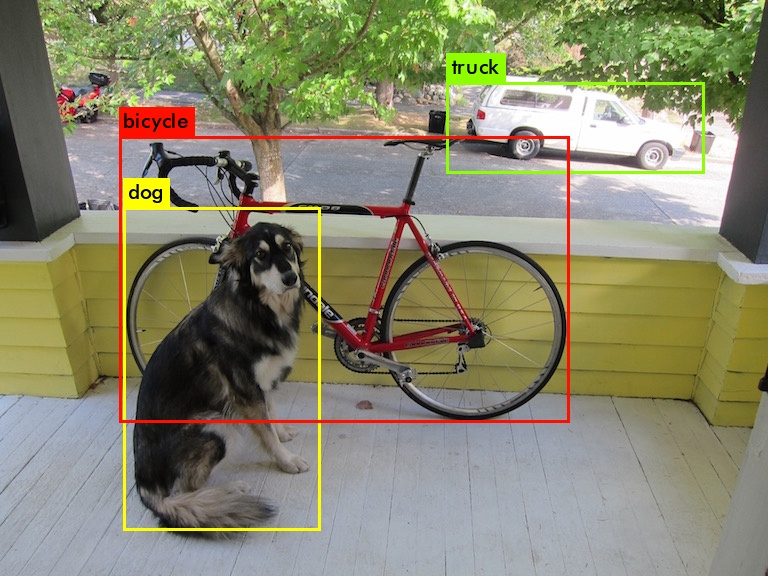
\includegraphics[height=3cm]{yolov2} 
  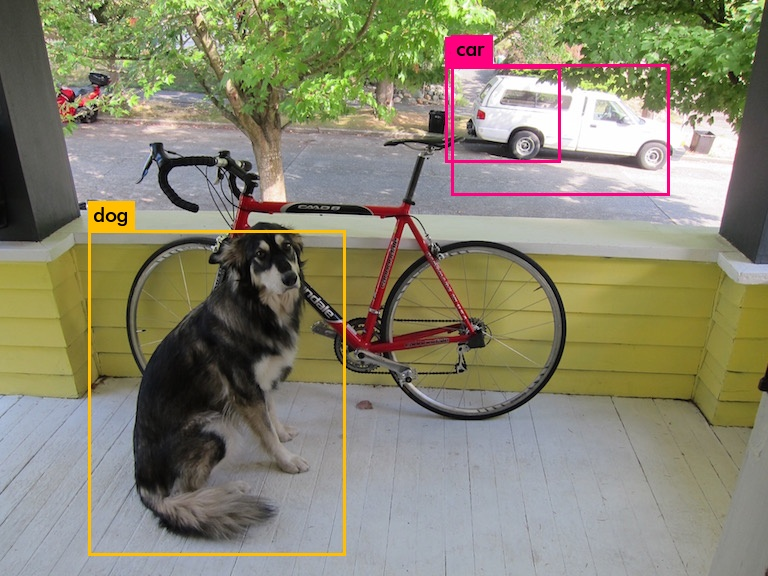
\includegraphics[height=3cm]{yolov2-tiny}
  \caption{Trade-off between accuracy and speed, left to right tested with Full-YOLO and Tiny-YOLO.}
  \label{fig:trade-off}
\end{figure}

\subsection{Training}
\label{subsec:training}

We explored two publicly-available datasets for training: the Caltech Pedestrian dataset \cite{caltech_peds} and the KITTI 2D Object Detection dataset \cite{kitti}. After testing our smaller YOLO models on the pedestrian dataset, we found that the algorithm performed poorly, likely due to the importance of small-scale features for detecting distant pedestrians being difficult to learn on such a small CNN frontend. Thus we put our full effort behind the KITTI dataset, which contains annotated images of cars around Karlsruhe, Germany. Four examples are shown in Figure~\ref{fig:kitti_examples}. Note that the vast majority of the training examples are cars viewed from an angle. Far fewer examples exist of a car directly in front of the camera. Our models all had difficulty detecting cars in this situation when applied to novel images collected in Boulder (see Figure~\ref{fig:detection_fails}).

\begin{figure}[p]
  \centering
  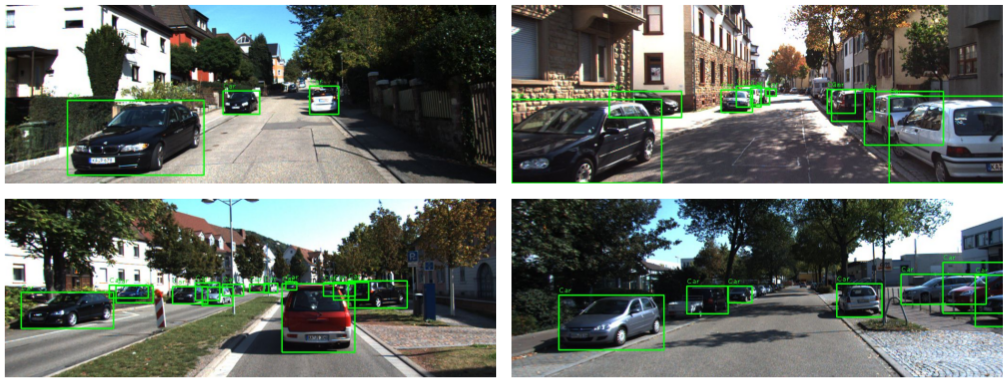
\includegraphics[width=0.8\textwidth]{kitti_examples}
  \caption{Examples of annotated training images provided by the KITTI dataset \cite{kitti}.}
  \label{fig:kitti_examples}
\end{figure}

\begin{figure}[p]
  \centering
  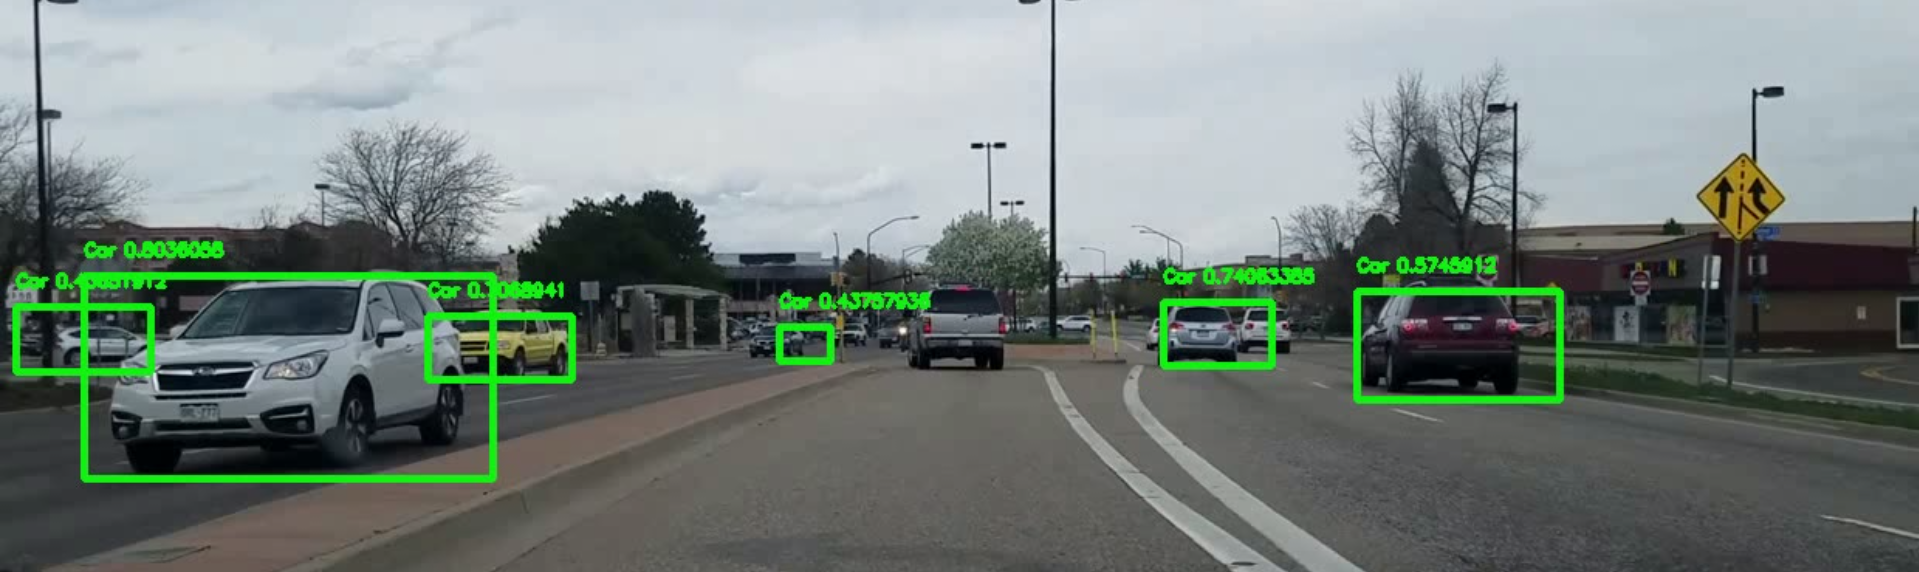
\includegraphics[width=0.7\textwidth]{fail_detect}
  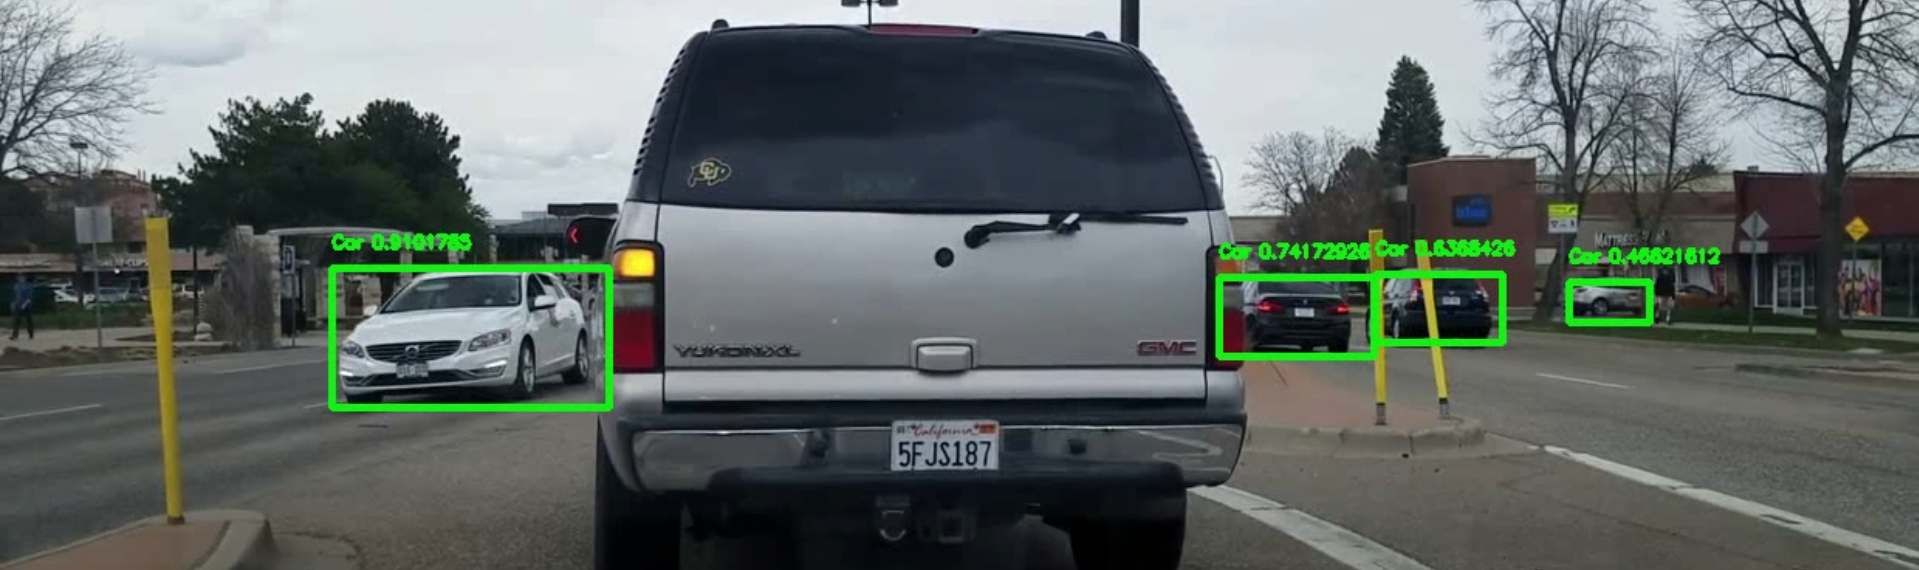
\includegraphics[width=0.7\textwidth]{fail_detect2}
  \caption{All YOLO networks we trained (MobileNet-YOLO is shown here) had trouble detecting cars directly in front of the camera; this is likely a consequence of the training data under-sampling this scenario.}
  \label{fig:detection_fails}
\end{figure}

\begin{figure}[p]
  \centering
  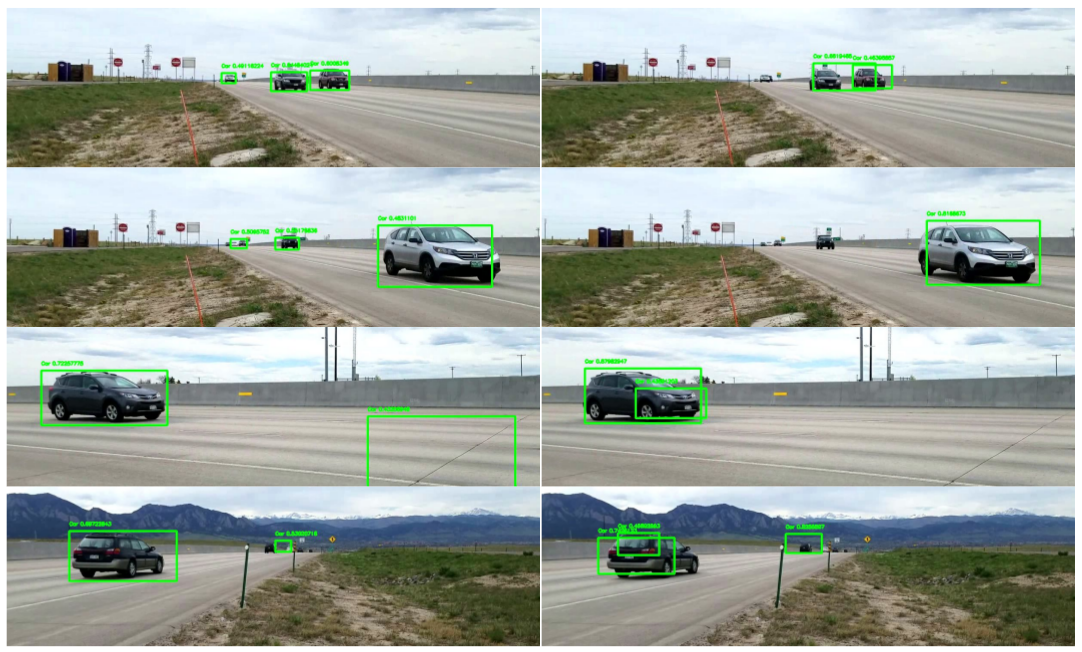
\includegraphics[width=0.8\textwidth]{boulder_results}
  \caption{Car detection in Boulder (at the overlook along U.S.\ Route 36) using MobileNet-YOLO (left) and Tiny-YOLO (right), both trained on the KITTI data.}
  \label{fig:boulder_results}
\end{figure}

We used a random sample of 2,400 of the 6,683 total KITTI images because they are just below the 2GB memory capacity of the Nvidia GTX 960 we used for training. We also performed image augmentation, with a random combination of Gaussian, average, and median blurring; sharpening; Gaussian noise; pixel dropout; and brightness and contrast adjustment. As will be shown in the results section, this allowed us to generalize reasonably well to data collected in Boulder. Training was conducted with early stopping, where the most-recent best-performing weights were saved after three training epochs failed to improve the validation accuracy.

\section{Results and Discussion}
\label{results}

We compare the original Tiny-YOLO architecture to the MobileNet-YOLO architecture, both qualitatively on our own dataset from driving around Boulder, and quantitatively on a validation set of 2,400 images sampled from the KITTI dataset (that were not used for training).

\begin{figure}[t]
  \centering
  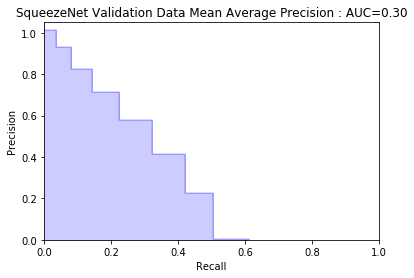
\includegraphics[width=0.32\textwidth]{pr_curve_squeezenet_kitti_validation}
  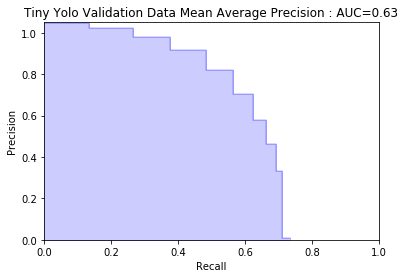
\includegraphics[width=0.32\textwidth]{pr_curve_tinyyolo_kitti_validation}
  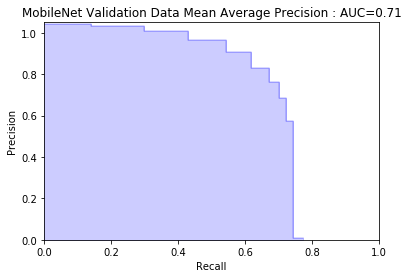
\includegraphics[width=0.32\textwidth]{pr_curve_mobilenet_kitti_validation}
  \caption{Precision-recall curves comparing network architectures, computed with validation set from KITTI data.}
  \label{fig:precition-recall}
\end{figure}

First, representative results of Tiny-YOLO and MobileNet-YOLO applied to some Boulder data are shown in Figure~\ref{fig:boulder_results}. Three key points are demonstrated in this figure. First, the KITTI dataset with the image augmentation described in Section~\ref{subsec:training} generalizes well to our ``in the wild'' data from driving around Boulder. Second, the MobileNet-YOLO we trained had a tendency to detect cars in empty patches of the roadway, whereas Tiny-YOLO often detected two cars where one existed. Third, MobileNet-YOLO gives much tighter bounding boxes and is able to pick out more distant vehicles than Tiny-YOLO.

While these results were qualitative and flashy, we also computed precision-recall curves from the KITTI data by varying the threshold for $P_{obj}$; they are are shown in Figure~\ref{fig:precition-recall}. Note that we also trained YOLO with a SqueezeNet front-end, which is an incredibly tiny CNN that does poorly on this object detection task, likely because of its small size. We include it in this figure for comparison's sake. Looking at their respective AUCs in Figure~\ref{fig:precition-recall}, MobileNet out-performs Tiny-Yolo on our validationdata. This is consistent with others' results (e.g. comparing Tiny Yolo and MobileNet's performance on the PASCAL VOC dataset \cite{mobilenet_on_voc}).

We should touch on the wall-time it takes to evaluate each of the networks we trained and compare them to the Full-YOLO network which is not feasible for mobile applications:
\begin{center}
\begin{tabular}{llll}
    & Full-YOLO & Tiny-YOLO & MobileNet-YOLO \\
CPU & 1.05 fps  & 2.16 fps  & 1.04 fps       \\
GPU & 10 fps    & 26 fps    & 23 fps        
\end{tabular}
\end{center}
We see that while MobileNet-YOLO is comparable to Full-YOLO with respect to frame rate on the CPU (a Xeon E5-2650 v3 @ 2.30GHz), its frame rate is comparable to Tiny-YOLO on a GPU, likely due to MobileNet's optimized architecture. This is particularly promising due to the superior performance of MobileNet-YOLO versus Tiny-YOLO as shown in Figures~\ref{fig:precition-recall} and \ref{fig:boulder_results}.

\begin{figure}[t]
  \centering
  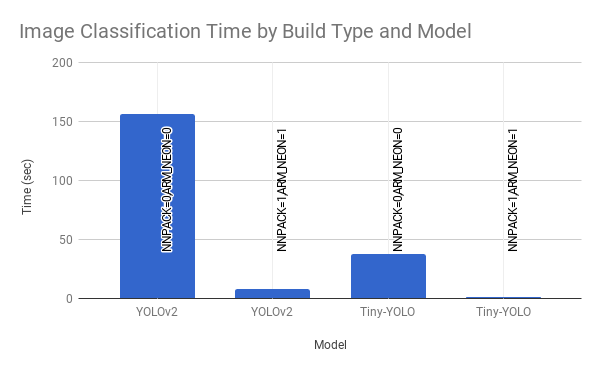
\includegraphics[width=0.6\textwidth]{images/hardware.png}
  \caption{Speed to evaluate a single image using different hardware optimizations.}
  \label{fig:hardware}
\end{figure}

Turning now to hardware optimization (refer to Figure~\ref{fig:hardware}), when we ran with all of the optimizations together, we were able to classify an image in approximately 1.2 seconds. This corresponds to a video stream classification rate of 0.83 fps. From the base case of 153 sec per image this is a roughly 115$\times$ decrease in classification time as shown in Figure~\ref{fig:hardware}. Overall, we were quite happy with this result. However, even after all of this, we were still only able to get to 0.8 fps which is not anywhere near the real time results we were targeting. Our conclusion is that in order to do real time object recognition, with our current hardware limitations, a GPU is absolutely necessary.

\section{Conclusion}
\label{conclusion}

While we did not achieve real-time object detection on a Raspberry Pi, we did explore a number of cost-saving measures. We successfully reduced the cost of detection by 115$\times$ on the Raspberry Pi by implementing various optimizations, and we showed that by using the MobileNet front-end we could achieve similar detection frame rates (slightly more than 20 fps) on a GPU to Tiny-YOLO but at increased accuracy. Ultimately, real-time detection on a low-cost platform is likely feasible with a GPU intended for mobile applications, but we were unable to explore this avenue due to cost and time constraints.

There are a number of ways this project could be extended in the future:
\begin{itemize}
\item Train the model on more datasets in addition to the current KITTI data such as Udacity self-driving car image data (we had trouble with this dataset due to its high resolution and thus massive file size). YOLO's excellent published results are partially due to the fact that the authors trained it on both VOC 2007 and 2012 with fine-tuning. In contrast, our model is primarily trained on only one relatively small dataset.

\item Play with the MobileNet parameters to explore the tradeoff between detection framerate and accuracy more thoroughly.

\item Incorporate motion detection into the network by concatenating two temporally adjacent images into an input tensor with six channels (RGB at time $t$, RGB at time $t-1$). One could also include an input node representing vehicle speed that is fully-connected to one of the early convolutional layers.

\item To further speed-up the hardware, we came across several compelling, low-cost solutions for deploying object recognition to the edge. One is the Movidius Neural Compute Stick by Intel \cite{Movidius_NCS}. It retails for about \$80 and can be added to the Raspberry Pi via USB. This accelerates Neural network applications and had demonstrated the ability to do object detection.

\item Another alternative is the Nvidia Jetson line of computers \cite{Nvidia_Tegra}. They're full SoCs with CPUs and GPUs specifically designed for embedded computing and machine learning. This would give us the ability to use CUDA to accelerate all the computations. The issue is that they're quite pricey for college students or home DIYers, ranging from \$500 and up. 
\end{itemize}

\bibliography{references}

\end{document}